\documentclass{ximera}

\newcommand{\RR}{\mathbb R}
\renewcommand{\d}{\,d}
\newcommand{\dd}[2][]{\frac{d #1}{d #2}}
\renewcommand{\l}{\ell}
\newcommand{\ddx}{\frac{d}{dx}}
\newcommand{\dfn}{\textbf}
\newcommand{\eval}[1]{\bigg[ #1 \bigg]}


%\outcome{Find tangent lines to parametric curves}
\author{Jim Talamo}

\begin{document}
\begin{exercise}

There are many ways to discuss first order differential equations.  When we study them, it's often useful to start with a predetermined convention that describes how to write them.  This exercise explores that idea.

In what follows, $x$ will be our independent variable, and $y$ will be the dependent variable.

\begin{exercise}
One common way to write a first order differential equation is in the form:

\[f(x,y,y')= 0 \]

Take a minute and think about what this is actually stating, then work the following:

For the differential equation:

\[
3xy'+x^2y=y^3+3x
\]
we have $f(x,y,y') = 3xy'+\answer{x^2y-y^3-3x}$.

\begin{hint}
To write the differential equation in the form $f(x,y,y')= 0$, all we have to do is move everything to the left-hand side, and call the left-hand side the function $f(x,y,y')$.
\end{hint}
\end{exercise}

\begin{exercise}
Another common way to write a first order differential equation is in the form:

\[\dd[y]{x}= f(x,y) \]

Take a minute and think about what this is actually stating, then work the following:

For the differential equation:

\[
3xy'+x^2y=y^3+3x
\]
we have $f(x,y) = \answer{\frac{y^3+3x-x^2y}{3x}}$.

\begin{hint}
To write the differential equation in the form $y' = f(x,y)$, all we have to do is solve for $\dd[y]{x}$ and call the righthand side the function $f(x,y)$.
\end{hint}

One advantage of this interpretation is that it allows us to think of the problem $\dd[y]{x}= f(x,y)$ as ``find a function $y(x)$ for which the slope of the tangent line at a point is found by evaluating $f(x,y)$ at that point.''

\begin{image}
  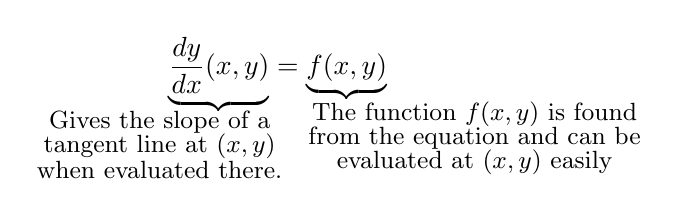
\begin{tikzpicture}
        \node at (0,0) {
          $\underbrace{\dd[y]{x}(x,y)}= \underbrace{f(x,y)}$};
        \node at (-1.5,-.6) {\small{Gives the slope of a }};
        \node at (-1.5,-.9) {\small{tangent line at $(x,y)$  }};
           \node at (-1.5,-1.2) {\small{when evaluated there.}};
        %%
          \node at (2.5,-.5) {\small{The function $f(x,y)$ is found}};
          \node at (2.5,-.8) {\small{from the equation and can be}};
            \node at (2.5,-1.1) {\small{evaluated at $(x,y)$ easily }};
      \end{tikzpicture}
  \end{image}

\begin{exercise}
We found we could write the equation:

\[
3x\dd[y]{x}+x^2y=y^3+3x
\]

in the form:

\[
\dd[y]{x} = \frac{y^3+3x-x^2y}{3x}
\]

The solution to this differential equation is:

\begin{multipleChoice}
\choice{A point $(x,y)$ for which $\dd[y]{x} = \frac{y^3+3x-x^2y}{3x}$}
\choice[correct]{A function for which the slope of the tangent line at any point $(x,y)$ is equal to $ \frac{y^3+3x-x^2y}{3x}$}
\end{multipleChoice}

Suppose that $y(x)$ is a solution to this differential equation.  Then, the slope of the tangent line to $y(x)$ at $(2,3)$ is $\answer{\frac{7}{2}}$

\begin{hint}
To find this, substitute $x=2$ and $y=3$ into $\frac{y^3+3x-x^2y}{3x}$
\end{hint}

One of the advantages of this representation of first order equations is that we can draw a \emph{direction field}.  To do this:

\begin{itemize}
\item[1.] Pick many different values for $(x,y)$ and find the slope of the tangent line associated to those values.
\item[2.] At each point $(x,y)$, draw a small portion of a line with that given slope.
\end{itemize}

The conceptual idea here is that functions are approximated by tangent lines near the point of tangency, so we can approximate the solutions to the differential equation by ``following the tangent lines''.

Of course, this is a painful process to do by hand, but thankfully, it is not so bad for computational software programs.  In fact, using a computer to draw the direction field this differential equation gives:


\begin{image}
{\def\length{sqrt(1+((y^3+3*x-x^2*y)/(3*x))^2)}
\begin{tikzpicture}
  \begin{axis}[
      xmin=-3, xmax=3,ymin=-3,ymax=3,domain=-3:3,view={0}{90},
      axis lines =center, xlabel=$x$, ylabel=$y$,
      every axis y label/.style={at=(current axis.above origin),anchor=south},
      every axis x label/.style={at=(current axis.right of origin),anchor=west},
      axis on top,
    ] 
    \addplot3 [penColor, quiver={u={1/\length}, v={(y^3+3*x-x^2*y)/(3*x)/(\length)},scale arrows=.2},samples=26] {0};
]  \end{axis}
\end{tikzpicture}}
\end{image}

\end{exercise}
\end{exercise}

\end{exercise}
\end{document}
